\newpage
\section{Thesis Conventions}
Every path mentioned in the thesis starts from the main path of the project repository.\\
We have two methods of separating the source code and code names from the text:
\begin{itemize}
    \item Inline code snippet:\\
    \texttt{puts("Hello World!");}
    \item Code listing:
\begin{lstlisting}[language=c++, caption=Example code snippet (./example\_dir/example\_file.cpp)]
std::cout << "Hello World!\n";
\end{lstlisting}
\end{itemize}
The paper consists of three main parts, theory starting from section \hyperref[sec:preface]{\ref*{sec:preface} Preface}, code description of TSEngine at section \hyperref[sec:code_descr]{\ref*{sec:code_descr} Code Description}, and ending starting with the section \hyperref[sec:problems]{\ref*{sec:problems} Problems During The Development}.

\newpage
\section{Abstract} 
\label{sec:preface}
\hspace{\parindent}
In the thesis, an architecture and implementation of a real-time graphics engine was created for virtual reality devices. To deepen the immersion of virtual reality experience, the software was extended to support an omnidirectional raceway adapted to VR. The work includes proprietary solutions for controlling the created environment with VR devices. The project is both a graphics engine and a game engine, it required theoretical knowledge of 3D graphics, and at the same time technical knowledge for the use of VR devices was necessary. Entity Component System and physics-based rendering (PBR) algorithm were implemented. The work begins with theoretical chapters outlining the theory and history of graphics and game engines, the history of virtual reality, and techniques that can be used when developing a graphics or game engine. The following chapters explain the mathematical part of implementing three-dimensional graphics on computer devices, show examples of how to test software. The next sections describe the technologies used in the implementation of the project, the step-by-step rendering process, the history, theory and mathematics behind PBR, the hardware that was used, and how the Cyberith Virtualizer Elite 2 docking raceway works. The next section is a description of the code, its extensibility. The next sections describe the problems that the authors of the work encountered, during the development of the project and the division of labor on the thesis. The thesis is finished with an epilogue and a discussion of possibilities for further development of TSEngine, and a conclusion.

Source code of this project is available at:\\
\href{https://github.com/damian-tomczak/tsengine}{https://github.com/damian-tomczak/tsengine}

Whereas prebuilt binaries of the project are available at (those executables were built with Release build configuration and are available in two variants with and without Virtualizer support):\\
\href{https://github.com/damian-tomczak/tsengine/releases}{https://github.com/damian-tomczak/tsengine/releases}

Non-compiled \LaTeX thesis is available at:\\
\href{https://github.com/damian-tomczak/beng_thesis}{https://github.com/damian-tomczak/beng\_thesis}

Instructions on how to build the code by oneself are detailed in the \hyperref[sec:how_to_run]{\ref*{sec:how_to_run} Instruction How To Build the Project} section. There is also a video presentation of the project available at \href{https://youtu.be/CxIDORRARdA}{https://youtu.be/CxIDORRARdA}

\begin{figure}[H]
  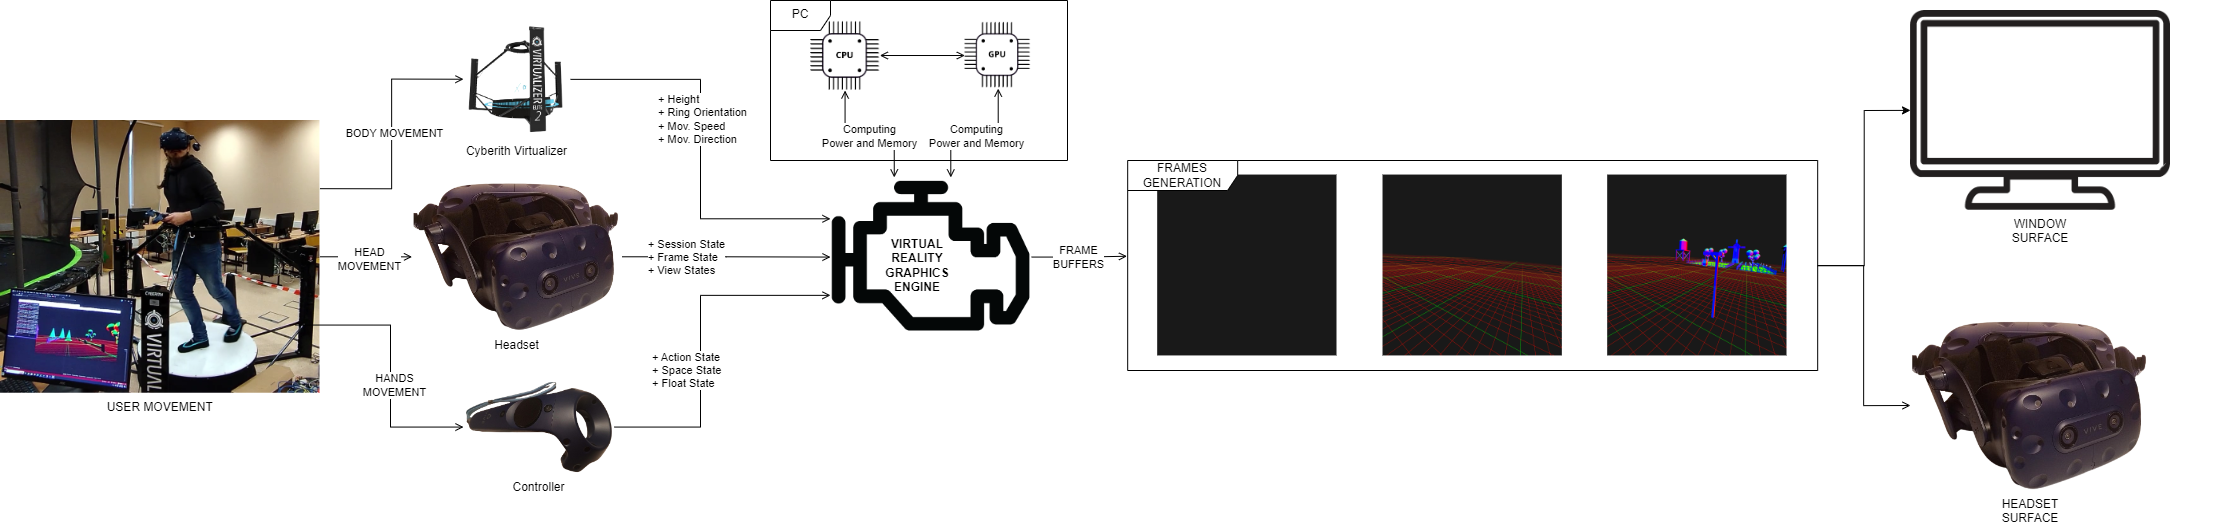
\includegraphics[width=\linewidth]{figures/graphicalAbstract.png}
  \caption{Graphical abstract, used image of Virtualizer from Cyberith  official page\cite{virtualizer_image}.}
\end{figure}


\newpage
\section{Streszczenie}
\hspace{\parindent}
W pracy stworzono architekturę i implementację silnika graficznego pracującego w czasie rzeczywistym, dla urządzeń wirtualnej rzeczywistości. Dla pogłębienia immersji zanurzenia się w wirtualnej rzeczywistości oprogramowanie zostało rozszerzone o obsługę bieżni dookólnej dostosowanej do VR. W pracy zawarto autorskie rozwiązania pozwalające na sterowanie w stworzonym środowisku za pomocą urządzeń VR. Projekt jest zarówno silnikiem graficznym, jak i growym, wymagał on wiedzy teoretycznej o grafice trójwymiarowej, a jednocześnie konieczna była wiedza techniczna do zastosowania urządzeń VR. Zaimplementowano Entity Component System oraz algorytmu renderowania bazującego na fizyce (PBR). Pracę rozpoczynają rozdziały teoretyczne przedstawiające teorię i historię silników graficznych i growych, historię wirtualnej rzeczywistości oraz techniki, które można wykorzystać podczas tworzenia silnika graficznego lub do gier. Następne rozdziały wyjaśniają część matematyczną implementacji trójwymiarowej grafiki na urządzeniach komputerowych, pokazują przykładowe sposoby testowania oprogramowania. Kolejne sekcje opisują technologie wykorzystywane w implementacji projektu, proces renderowania krok po kroku, historię, teorię i matematykę dotyczącą PBR, sprzęt, który został użyty, oraz sposób, w jaki działa Cyberith Virtualizer Elite 2 - bieżnia dookólna. Kolejna sekcja to opis kodu, możliwości jego rozszerzania. W następnych sekcjach opisano problemy, z jakimi zetknęli się autorzy pracy, podczas rozwoju projektu i podział pracy nad pracą dyplomową. Pracę wieńczy epilog i dyskusja o możliwościach dalszego rozwoju TSEngine, oraz podsumowanie.


Kod źródłowy tego projektu jest dostępny pod adresem:\\
\href{https://github.com/damian-tomczak/tsengine}{https://github.com/damian-tomczak/tsengine}

Podczas gdy już przekompilowane są dostępne w wariencie Release'owym z ogsługą Virtualizer'a lub bez:\\
\href{https://github.com/damian-tomczak/tsengine/releases}{https://github.com/damian-tomczak/tsengine/releases}

Nie przekompilowana praca dyplomowa w formacie \LaTeX jest dostępna pod adresem:\\
\href{https://github.com/damian-tomczak/beng_thesis}{https://github.com/damian-tomczak/beng\_thesis}

Instrukcja odnośnie wybudowania kodu jest dostępna w rozdziale \hyperref[sec:how_to_run]{\ref*{sec:how_to_run} Instruction How To Build the Project}. Dostępna jest również prezentacja wideo pod adresem \href{https://youtu.be/CxIDORRARdA}{https://youtu.be/CxIDORRARdA}

\begin{figure}[H]
  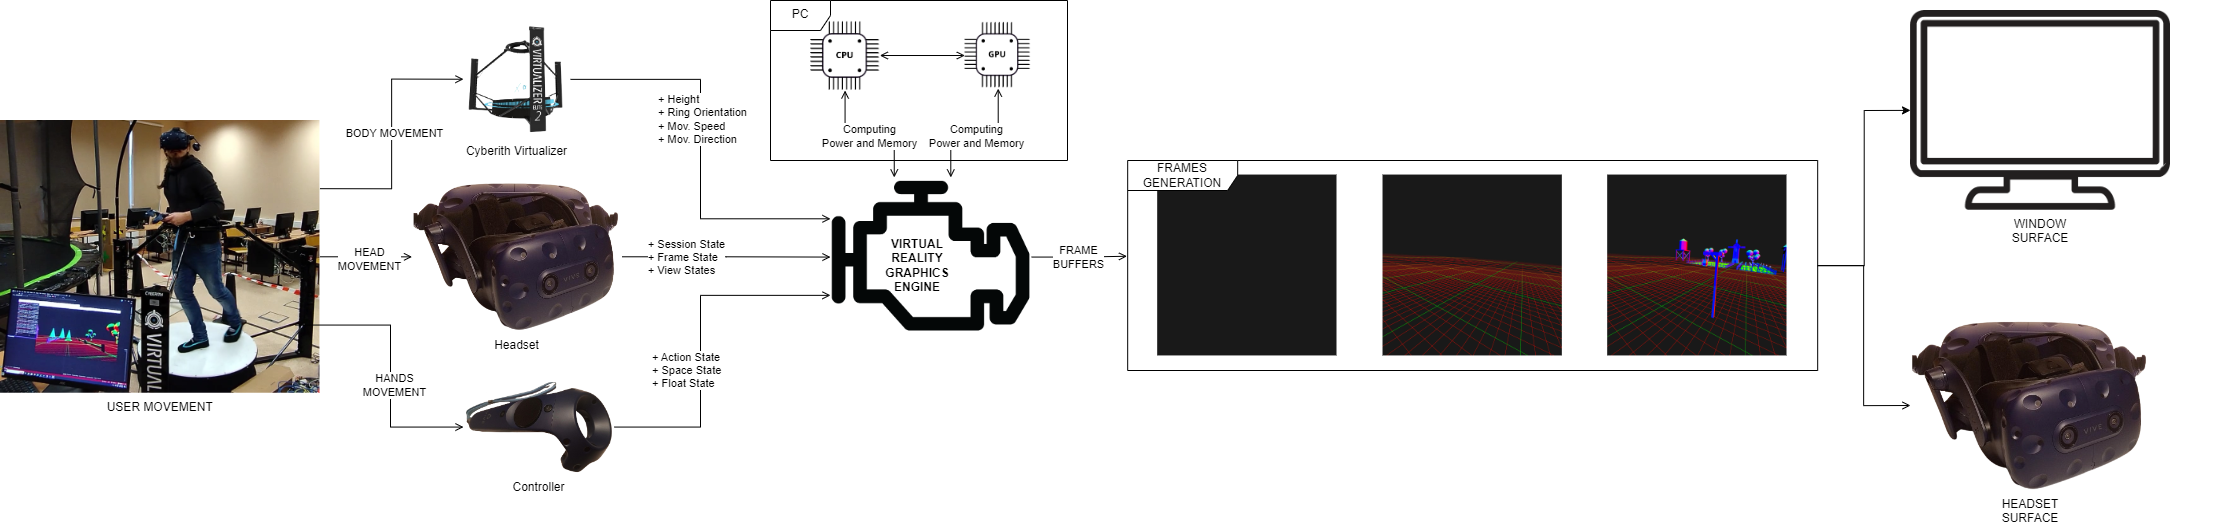
\includegraphics[width=\linewidth]{figures/graphicalAbstract.png}
  \caption{Abstrakt graficzny, użyty obrazek Virtualizera z oficjalnej strony Cyberith\cite{virtualizer_image}.}
\end{figure}

